\documentclass[tikz,dvipsnames]{standalone}
\usepackage[]{xcolor}
\PassOptionsToPackage{dvipsnames}{xcolor}
\usepackage[utf8]{inputenc}
\usepackage[]{xcolor}
\usepackage{amsmath}
\usepackage{amssymb}

\usetikzlibrary{arrows,positioning,shapes}
\usetikzlibrary{arrows.meta,positioning,shapes}
\usetikzlibrary{decorations.pathreplacing,decorations.markings}
\usetikzlibrary{calc}
\tikzset{
  % style to apply some styles to each segment of a path
  on each segment/.style={
    decorate,
    decoration={
      show path construction,
      moveto code={},
      lineto code={
        \path [#1]
        (\tikzinputsegmentfirst) -- (\tikzinputsegmentlast);
      },
      curveto code={
        \path [#1] (\tikzinputsegmentfirst)
        .. controls
        (\tikzinputsegmentsupporta) and (\tikzinputsegmentsupportb)
        ..
        (\tikzinputsegmentlast);
      },
      closepath code={
        \path [#1]
        (\tikzinputsegmentfirst) -- (\tikzinputsegmentlast);
      },
    },
  },
  % style to add an arrow in the middle of a path
  mid arrow/.style={postaction={decorate,decoration={
        markings,
        mark=at position .5 with {\arrow[#1]{stealth}}
      }}},
  % style to add an arrow at a position of a path
  arrow at/.style 2 args={postaction={decorate,decoration={
        markings,
        mark=at position #1 with {\arrow[#2]{stealth}}
      }}},
}

\tikzset{cross/.style={cross out, draw=black, minimum size=2*(#1-\pgflinewidth), inner sep=0pt, outer sep=0pt},
%default radius will be 1pt. 
cross/.default={1pt}}

\begin{document}
  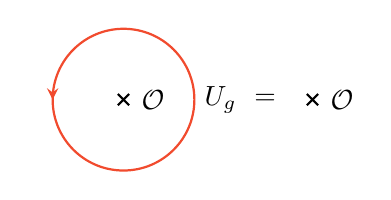
\begin{tikzpicture}[thick]
    \pgfmathsetmacro{\rad}{.9}
    \coordinate (O) at (0,0);
    \node[cross=.1cm] at (O) {};
    \node[anchor = west,xshift=.1cm] at (O) {$\mathcal{O}$};
    \draw[color=RedOrange,mid arrow] (\rad,0) arc (0:360:\rad);
    \node[anchor = west] at (\rad,0) {$U_g$};
    \node at (-1.1,0) {};
    \node at (\rad+.9,0) {$=$};
    \coordinate (O2) at (\rad+1.5,0);
    \node[cross=.1cm] at (O2) {};
    \node[anchor = west,xshift=.1cm] at (O2) {$\mathcal{O}$};
  \end{tikzpicture}
\end{document}
